\chapter{Tworzenie polskich zbiorów}
W ostatnim czasie w szczególności nacisk zostaje przenoszony z modeli na odpowiednie przygotowanie i jakość zbiorów danych. Przykładem tego jest wydany w ostatnim czasie artykuł \bibtitle{Textbooks are all you need} \mycite{Gunasekar2023}, który demonstruję jak dużą poprawę można uzyskać bez powiększania i komplikowania wykorzystywanego modelu, lecz poprzez stworzenie wysokiej jakości zbioru danych.

Jako, że dla zadania \code{Text-to-SQL} na moment pisania niniejszej pracy nie istnieją żadne zbiory danych w języku polskim, a także ze względu na duże ich znaczenie, wiele uwagi zostało poświęcone tej kwestii. 

Na początku bieżącego rozdziału omówione zostaną przyjęte założenia dotyczące tworzenia polskich zbiorów, a następnie przedyskutowane dokładnie dwa kluczowe dla tego procesu elementy: dynamiczne generowanie oraz sposób dokonywania tłumaczenia. Ostatecznie nastąpi analiza i podsumowanie stworzonych zbiorów.

\section{Przyjęte założenia}
Po przeanalizowaniu różnic pomiędzy istniejącymi tłumaczeniami zbioru \code{Spider} określone zostały założenia przyjęte na potrzebę stworzenia zbiorów polskich.

% To fix:
Podczas tłumaczenia zbiorów przyjęto dwa podstawowe założenia. Pierwszym jest wykorzystanie tłumaczenia maszynowego, zamiast manualnego. Drugi stanowi dynamiczne generowanie finalnych zbiorów zamiast jednorazowego tłumaczenia wszystkich przykładów i udostępnienia jedynie zmodyfikowanej ich wersji. Oba założenia zostaną rozwinięte, uzasadnione i dokładnie przedyskutowane w poniższych dwóch sekcjach.

\subsection{Tłumaczenie maszynowe}
Pomimo wskazanej w sekcji \ref{text:translation-method} dominacji tłumaczenia manualnego nad maszynowym postanowiono wykorzystać to ostatnie. Przyczyn tej decyzji jest kilka. Przede wszystkim w realizację tłumaczenia aktywnie zaangażowana jest tylko jedna osoba, w odróżnieniu do wcześniejszych prac, w których w tym procesie uczestniczyło ich kilka, a w przypadku rosyjskiego zbioru nawet profesjonalny tłumacz. Drugą przesłanką jest ograniczony czas, ze względu na pracę magisterką w ramach której niniejszy temat jest realizowany. Ostatecznie jest to zadanie żmudne, a zbiór maszynowy, pomimo niższej jakości, także pozwoli, a nawet da więcej czasu, na wykonanie eksperymentów.

\subsection{Generowanie zbiorów}
Wszystkie dotychczasowe tłumaczenia zbioru Spider sprowadzają się jedynie do udostępnienia zmodyfikowanej wersji zbioru, bez żadnych dodatkowych skryptów. Wydaje się to wystarczające i dla większości zastosowań w rzeczywistości jest. Taki zbiór stanowi bardzo dobry benchmark służący do porównywania różnych algorytmów, ponieważ nie ma żadnych niedomówień w kwestii jego zawartości.

W niniejszej pracy zaproponowano dość innowacyjne, bo niespotykane we wcześniejszych zbiorach podejście, polegające na skryptowym generowaniu zbiorów w żądanej konfiguracji. Na początku zostaną one rozbite na elementarne składniki, czyli pytania, zapytania SQL oraz schematy baz danych. Następnie będzie można przeprowadzić syntezę tych komponentów w kompletny zbiór wybierając przy tym język pytań, język zapytań oraz jedną z możliwych wersji schematu baz danych.

Zdecydowano się na opracowanie takiej metody, gdyż zauważono, że ma ona szereg zalet. Po pierwsze nie trzeba decydować się czy tłumaczyć nazwy tabel i kolumn, czy nie, jak to robili dotychczasowi autorzy tłumaczeń, a nie byli co do tego zgodni. Opisanym sposobem można stworzyć kilka mapowań starych nazw na nowe i do syntezy wykorzystać to, które będzie w danym przypadku najlepsze. Jest to poza zakresem pracy, ale znacząco to ułatwia również tłumaczenia zbioru na inne języki, bo wszystkie komponenty zostały już rozplątane. Generalnie taka strategia jest bardzo elastyczna i otwiera drogę na nowe eksperymenty.

\subsection{Tłumaczenie zbiorów pokrewnych}
Oprócz przetłumaczenia zbioru \code{Spider} postanowiono dokonać tego również dla czterech zbiorów pokrewnych przedstawionych wcześniej w sekcji \ref{text:related-datasets}. Prostym powodem tego jest chęć zdobycia większej liczby próbek w nadziei, że pozwoli to finalnie na wytrenowali lepszej jakości modeli. Poza tym przetłumaczenie \code{Spider-Syn} oraz \code{Spider-DK} pozwoli na testowanie tworzonych algorytmów pod kontem odporności na synonimy, czy znajomości wiedzy domenowej. 

Przetłumaczenie dodatkowych zbiorów jest ułatwione, ponieważ dzięki współdzielonym bazą danych translacji nazw tabel i kolumn wystarczy dokonać jednorazowo. Zastosowane podejście polegające na skryptowym generowaniu ostatecznych zbiorów jeszcze bardziej uprasza ten proces, więc postanowiono to wykorzystać. Nie znaleziono informacji na temat wcześniejszych prób tłumaczenia tych zbiorów, więc niniejsza praca być może jest pierwsza.

\subsection{Oryginalna zawartość baz danych}
Zawartość baz danych postanowiono pozostawić bez zmian - ewentualnemu tłumaczeniu podlegać będzie jedynie ich schemat. Powodem do tego jest duża ilość znajdujących się tam informacji, których tłumaczenie maszynowe skutkowałoby naliczeniem istotnych opłat. Jest to jednocześnie działanie pokrywające się z większością istniejących podejść do tłumaczenia zbioru \code{Spider}. Pomimo pozostawienia oryginalnej zawartości baz danych, modele trenowane na nich wciąż są w stanie osiągać wysokie wyniki, co potwierdza słuszność tego podejścia.

\section{Przygotowanie zbiorów angielskich}
Poza angielskim zbiorem \code{Spider}, którego przetłumaczenie bez wątpienia było najistotniejsze, przetłumaczono również zbiory \code{Spider-Syn}, \code{Spider-DK}, \code{SParC} oraz \code{CoSQL}. Ich struktura oraz przeznaczenie znacząco odbiega od zbioru \code{Spider} i aby je wykorzystać podjęte zostały dodatkowe kroki, które zostały w niniejszej części podsumowane. Niektóre z nich były konieczne, jak zamiana zbiorów z kontekstowych na bezkontekstowe, a inne opcjonalne, jak deduplikacja poprawiająca efektywność nauki modeli. Kroki te sprawiają jednak, że tłumaczenia owych dodatkowych zbiorów nie stanowią idealnych odpowiedników oryginałów. W różnym stopniu, ale należy traktować je jako nowe zbiory i unikać zestawiania osiąganych na nich rezultatów z angielskimi oryginałami.

\subsection{Konwersja zbiorów kontekstowych na bezkontekstowe}
W ramach realizowanego tematu rozważany jest problem tłumaczenia bezkontekstowego, co jest pozornie sprzeczne z wykorzystaniem zbiorów \code{SParC} oraz \code{CoSQL}. Nie zawierają one bowiem prostego szeregu pytań i odpowiadających im zapytań SQL, lecz dodatkowo porządkują je w konwersacje, gdzie kolejne wiadomości bazują na znajomości poprzednich. Zauważono, jednak że zbiory kontekstowe mogą zostać przekonwertowane na bezkontekstowe poprzez wybranie z każdej konwersacji jedynie pierwszego pytania i odpowiedzi. Nie istnieje wówczas żadna historia wcześniejszych wiadomości, więc takie przykłady nie posiadają żadnego dodatkowego kontekstu. Powstałe w ten sposób zbiory znacznie różnią się od oryginalnie kontekstowych zbiorów \code{SParC} oraz \code{CoSQL}, więc całkowicie nieuzasadnionym by było zestawianie ze sobą osiąganych na nich wyników.

\subsection{Modyfikacja pytań}
Część pytań wewnątrz zamienionych już na bezkontekstowe zbiorów \code{SParC} oraz \code{CoSQL} wyraźnie odróżniała się od reszty. Zawierały one bowiem wyrażenia charakterystyczne dla konwersacji, takie jak \enquote{Hi}, \enquote{Hello}, \enquote{How are you}. Są one dla rozważanego problemu niepożądane, bo nie stanowią typowych pytań, które użytkownik wprowadziłby do systemu wiedząc, że zwraca on jedynie zapytania SQL. Z tego powodu postanowiono znaleźć takie wystąpienia za pomocą wyrażeń regularnych oraz funkcji wyszukiwania dostępnej wewnątrz wykorzystywanego edytora i usunąć niepotrzebne fragmenty.

\subsection{Deduplikacja w obrębie zbiorów}
Jako zduplikowane zostały uznane przykłady, które posiadają identyczną bazę danych oraz takie same znormalizowane angielskie pytania (przekonwertowane na małe litery i bez niepotrzebnych białych znaków). Deduplikacji w obrębie zbiorów dokonano poprzez zwyczajne usunięcie występujących kilkukrotnie próbek. Okazało się, że znaleziono takie w każdym ze zbiorów, poza \code{Spider-DK}. 25 przypadków zostało zlokalizowanych nawet w samym zbiorze \code{Spider}, lecz w nim modyfikacji nie wprowadzano, bo ze względu na jego wysoką renomę chciano, by próbki w polskim wariancie dokładnie mu odpowiadały. Najwięcej duplikatów zostało znalezionych w zbiorze \code{SParC}. Widocznie w tym oryginalnie kontekstowym zbiorze wiele konwersacji rozpoczynało się od tych samych wiadomości i różnice następowały dopiero później.

\subsection{Deduplikacja pomiędzy zbiorami}
Istotnym problemem okazały się duplikaty pomiędzy zbiorami. W większości występowały one między \code{Spider}, a całą resztą, ponieważ \code{Spider} powstał jako pierwszy. Widać to doskonale na rysunku \ref{fig:deduplication-before}, gdyż największa liczba duplikatów znajduje się w wierszu oraz kolumnie odpowiadającej właśnie zbiorowi \code{Spider}. Dużą liczbą powtórzeń wyróżnia się w szczególności para zbiorów \code{Spider} oraz \code{Spider-Syn}, ponieważ w tym ostatnim autorzy umieszczali oryginalną próbkę, jeżeli nie udało im się wymyślić rozsądnego synonimu. Ostatecznie całą duplikację ze zbiorem \code{Spider} postanowiono usunąć. Jedynym wyjątkiem są powtórzenia pomiędzy parą \code{Spider-DK} oraz \code{Spider}, które pozostawiono, ponieważ \code{Spider-DK} ma charakter czysto walidacyjny i 206 znalezionych duplikatów to nie przypadkowe próbki, lecz precyzyjnie wyselekcjonowane ze zbioru \code{Spider} przykłady zawierające wiedze domenową. Pozostawioną w zbiorach duplikację po usunięciu części próbek przedstawiono na rysunku \ref{fig:deduplication-after}. 

\begin{figure}[ht!]
\centering
\begin{subfigure}{0.49\textwidth}
    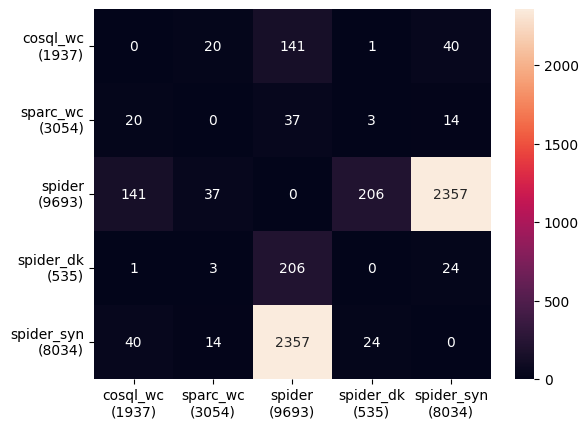
\includegraphics[width=\textwidth]{images/duplicates_before.png}
    \caption{Przed deduplikacją}
    \label{fig:deduplication-before}
\end{subfigure}
\hfill
\begin{subfigure}{0.49\textwidth}
    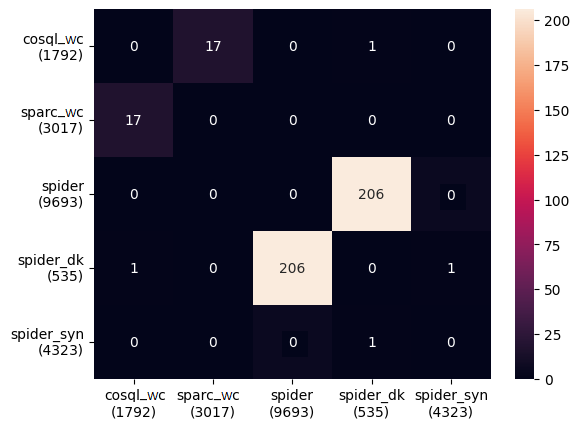
\includegraphics[width=\textwidth]{images/duplicates_after.png}
    \caption{Po deduplikacji}
    \label{fig:deduplication-after}
\end{subfigure}
\caption[Diagramy ilustrujące liczbę duplikatów pomiędzy zbiorami]{Diagramy ilustrujące liczbę duplikatów pomiędzy zbiorami - na osiach umieszczono nazwy zbiorów wraz z liczbą próbek, a wartości w komórkach macierzy wskazują liczbie duplikatów pomiędzy daną parą zbiorów.}
\label{fig:cross-dataset-duplicates}
\end{figure}

\subsection{Deduplikacja tłumaczeń}
Deduplikacja tłumaczeń to działanie, które dotyczy wyłącznie zbioru \code{Spider-Syn}. Trzeba zauważyć, że opisane powyżej usuwanie duplikatów bazuje na angielskich wersjach pytań, co wydaję się wystarczające, ponieważ jeżeli pytania angielskie się różnią, to ich polskie tłumaczenia również powinny się różnić. W przypadku próbek zawartych w zbiorze \code{Spider-Syn} jest jednak często inaczej. Dla przypomnienia, zawiera on próbki z oryginalnego zbioru \code{Spider}, lecz z wybranymi słowami zamienionymi na synonimy. Okazuje się, że te synonimy oraz bazowe słowa od których pochodzą tłumaczone są niejednokrotnie przez \code{DeepL} na te same polskie wyrażenia, co skutkuje duplikatami w liczbie 1350. Proces ich powstawania został zilustrowany na rysunku \ref{fig:deduplication-after-translation}. Aby pozbyć się tak powstałej duplikacji postanowiono usunąć niepotrzebne próbki ze zbioru \code{Spider-Syn}. Działanie to, w odróżnieniu do wcześniej opisanych, musiało się odbyć już po dokonaniu tłumaczenia na język polski.

\begin{figure}[ht!]
  \centering
  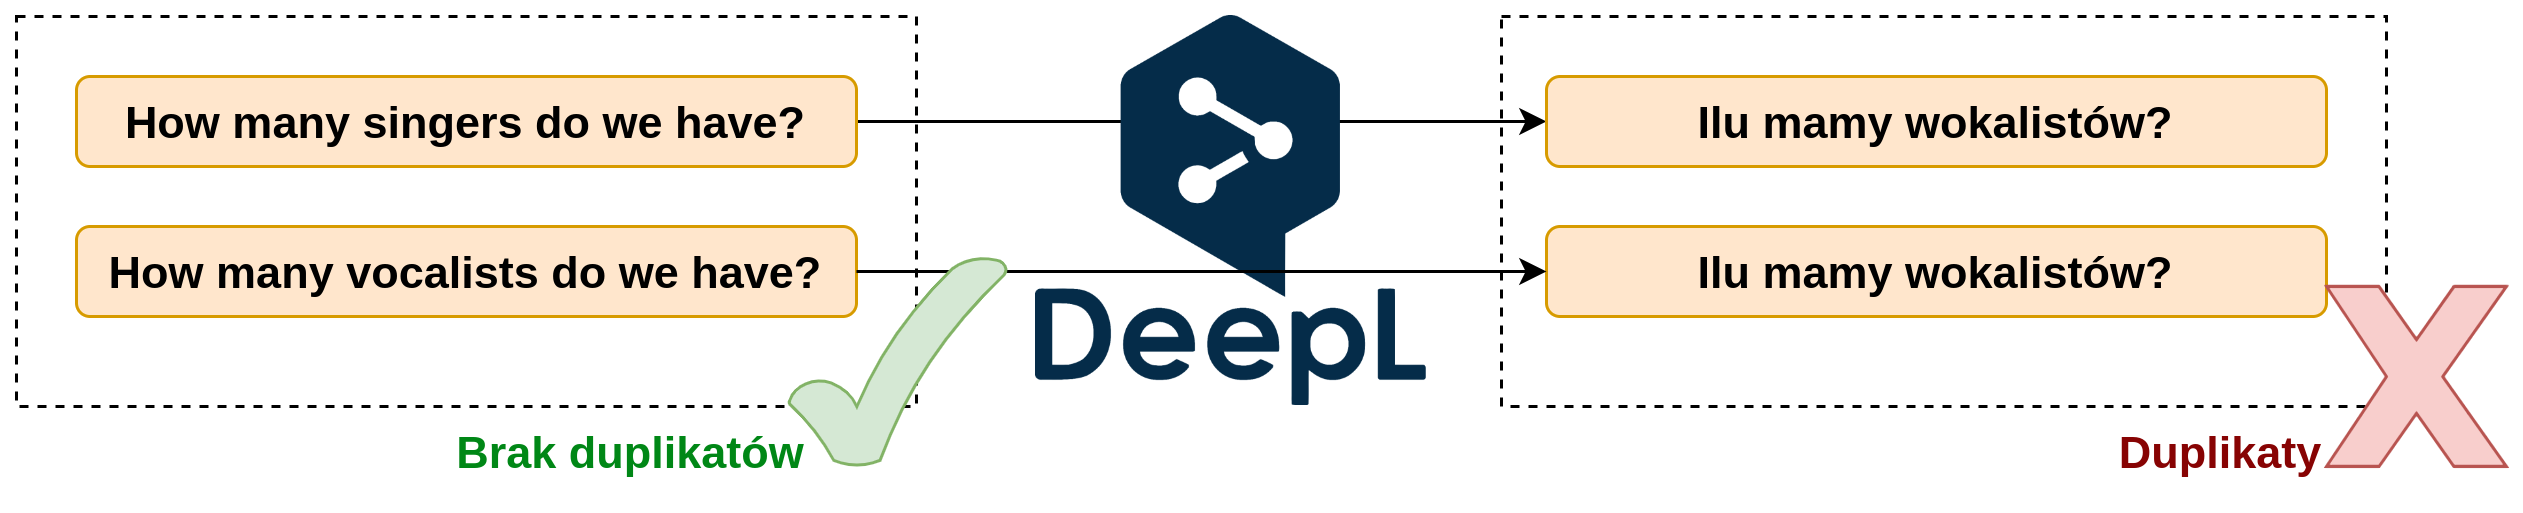
\includegraphics[width=1.0\linewidth]{images/duplication_after_translation.png}
  \caption[Sposób powstawania duplikacji w wyniku tłumaczenia]{Sposób powstawania duplikacji pomiędzy \code{Spider} i \code{Spider-Syn} w wyniku tłumaczenia}
  \label{fig:deduplication-after-translation}
\end{figure}

\section{Generowanie zbiorów}
Generowanie zbiorów w różnych konfiguracjach, czy też inaczej synteza zbiorów, jest ważnym elementem niniejszej pracy i w znaczny sposób odróżnia ją od wcześniejszych podejść. W związku z tym zostanie ono w tej części dokładnie opisane.

Implementacja tej strategii sprowadza się do stworzenia skryptu pozwalającego na wygenerowanie zbioru o żądanych parametrach. Wśród nich możliwe jest określenie języka pytań, języka wartości w zapytaniach i wariantu tłumaczenia schematu bazy danych.

Proces syntezy posiada dwa główne etapy: zmianę nazw tabel i kolumn oraz rekonstrukcję informacji redundantnych. Zostaną one dokładnie opisane w osobnych sekcjach. Wcześniej natomiast omówione zostaną dane źródłowe, które potrzebne są do przeprowadzenia wspomnianych etapów.

\subsection{Dane źródłowe}
Przed przystąpieniem do tworzenia skryptu generującego zbiory w żądanych konfiguracjach konieczne okazało się zastanowienie nad danymi źródłowymi, które będą niezbędne do jego działania. Ostatecznie dane te zostały rozbite na dwa typy plików: próbki, które zawierają alternatywne wersję pytań i zapytań SQL oraz pliki mapowań nazw schematów, które zawierają kompletne mapowania oryginalnych nazw tabel i kolumn na nowe. Formaty tych plików zostały opisane w poniższych sekcjach. Taka dekompozycja umożliwia dodawanie kolejnych zbiorów poprzez tworzenie nowych plików próbek i dodawanie kolejnych sposobów tłumaczenia nazw tabel i kolumn poprzez tworzenie nowych plików mapowania.

\subsubsection{Plik próbek}
Przykładowy element z opracowanego pliku próbek został przedstawiony na listingu \ref{lst:new-sample}. Ma on stanowić bazę na podstawie której będą generowane kompletne zbiory. Każdy zawarty w nim przykład zawiera jedynie niezbędne informacje, czyli nazwę bazy danych oraz alternatywne warianty pytań i zapytań SQL. Przedstawiony przykład zawiera jedynie angielskie i polskie warianty, bo tylko one są istotne dla realizacji niniejszego tematu. Nic nie stoi na przeszkodzie, aby dodać jednak kolejne języki, gdyż zarówno format omawianego pliku, jak i skrypt generujący został na taką okoliczność przygotowany.

\begin{minipage}{\linewidth}
\lstinputlisting[
style=json,
caption=Pojedynczy przykład z pliku próbek stanowiącego dane źródłowe,
label={lst:new-sample},
]{listings/new_sample.json}
\end{minipage}

Warto zwrócić uwagę, że próbki w finalnym zbiorze muszą posiadać znacznie więcej atrybutów niż te przedstawione powyżej. Powinny zawierać dodatkowo pytania i zapytania SQL podzielone na tokeny oraz sparsowane zapytania. Są to jednak w dużej części informacje redundantne, które można z powodzeniem odtworzyć na podstawie skromnych informacji przedstawionych powyżej i jest to jedna z funkcji które będzie realizował skrypt generujący. Sprawia to, że tworzone rozwiązanie jest zgodne z powszechnie cenioną architekturą \code{Single Source of Truth} (SSOT). Polega ona na unikaniu za wszelką cenę powielania tych samych informacji w kilku miejscach, ponieważ, gdy zostaną zmodyfikowane to pojawia się bardzo duże ryzyko powstania niespójności. Istotność tej metodyki w inżynierii oprogramowania została dobrze przedstawiona w artykule \bibtitle{Single Source of Truth (SSOT) for Service Oriented Architecture (SOA)} \mycite{Pang2014}.

\subsubsection{Plik mapowania nazw}
Aby umożliwić dokonywanie różnych tłumaczeń schematów baz danych, czyli nazw tabel i kolumn, opracowany został format pliku przedstawiony na listingu \ref{lst:new-trans}. Zawiera on informacje pozwalające na dokonanie mapowania oryginalnych nazw na dowolne inne. Jest to plik json o kilku stopniach zagnieżdżenia. Na najwyższym poziomie jest słownikiem, który dla każdej nazwy bazy danych zawiera listę tabel, a każda tabela listę kolumn. Wszystkie obiekty reprezentujące tabele i kolumny posiadają źródłowe oraz docelowe nazwy na jakie powinny zostać przetłumaczone. Jak już wiadomo mają one dwa rodzaje nazw, które zostały tutaj uwzględnione: oryginalnie występujące w bazach danych oraz odpowiedniki w języku naturalnym.

\begin{minipage}{\linewidth}
\lstinputlisting[
style=json,
caption=Fragment opracowanego pliku mapowań nazw schematu,
label={lst:new-trans},
]{listings/new_trans.json}
\end{minipage}

Należy zwrócić uwagę, że zaproponowany format pozwala, aby dana nazwa kolumny była tłumaczona na różne sposoby w zależności od tabeli i bazy w której się znajduję. Podobnie ta sama nazwa tabeli może być tłumaczona na różne sposoby w zależności od zawierającej ją bazy danych. Jest to celowy zabieg i wymagany w celu umożliwienia prawdziwie wysokiej jakości tłumaczenia. Rozważmy dla przykładu tabelę o nazwie \code{department}. W bazie dotyczącej biznesu prawdopodobnie powinna zostać przetłumaczona jako \code{dział}, natomiast w domenie uniwersyteckiej jako \code{wydział}. Przyjęcie bardziej zaawansowanego podejścia umożliwiło dokonanie tego typu kontekstowego tłumaczenia, przedstawionego w dalszej części pracy.

\subsection{Zmiana nazw tabel i kolumn}
Zmiana nazw tabel i kolumn zgodnie z określonym mapowaniem to dla opracowanego procesu generowania zbiorów najważniejszy punkt. Sprowadza się on do dokonania dwóch rodzajów modyfikacji, opisanych szczegółowo poniżej. Prostszy rodzaj to podmiana nazw w samych bazach danych \code{SQLite}. Znacznie trudniejsze okazało się jednak dokonanie modyfikacji w zapytaniach. Powstały one przecież na bazie oryginalnych nazw tabel i kolumn, które należało wychwycić i podmienić na nowe.

% Zmiana nazw w schematach to zmiana nazw tabel i kolumn zgodnie z określonym mapowaniem nazw schematów, które jest określone za pomocą wprowadzonego wcześniej pliku.

% Dokonanie zmian nazw w schemacie, z punktu widzenia oryginalnego zbioru Spider, sprowadza się do zmodyfikowania dwóch elementów: samych baz danych oraz schematu wewnątrz zapytań SQL. W poniższych sekcjach zostanie przedstawiony opracowany algorytm, który tego dokonuje wraz z analizą alternatywnych możliwości. 

\subsubsection{Modyfikacje w bazach danych}
Zmodyfikowanie nazw tabel i kolumn w bazach danych nie stanowi dużego wyzwania, ponieważ wystarczy wykonać na każdej z nich serię instrukcji typu \sql{ALTER TABLE}. Przystępując do tego należy jednak upewnić się, że zastosowanie danego mapowanie nie tworzy konfliktujących ze sobą pod względem nazw elementów, bo wówczas operacja się nie powiedzie. Aby to sprawdzić oraz zlokalizować miejsca ewentualnych kolizji stworzony został skrypt, który analizuje podane mapowanie pod tym kątem. Podczas tłumaczenia zauważono także, że należy pomijać tabele o nazwie \code{sqlite\_sequence}, ponieważ jest to specjalna tabela i jej modyfikacja nie jest możliwa.

\subsubsection{Modyfikacje w zapytaniach}
Dokonanie podmiany nazw tabel i kolumn w zapytaniach SQL stanowi najtrudniejszy etap w całym procesie generowania zbiorów. Przyczyną tego jest przyjęte podejście polegające na tym, że dana kolumna może być przetłumaczona na różne sposoby, w zależności od tabeli w której się znajduję. W przypadku modyfikacji baz danych było oczywistym do której tabeli należy każda kolumna, bo wynika to z ich jasno zdefiniowanej struktury. Zapytania SQL są natomiast w gruncie rzeczy zwykłym tekstem i wydobycie z nich kolumn oraz ustalenie tabel do których należą stanowi duże wyzwanie.

Najłatwiejsze podejście do tego problemu, ale posiadające istotny problem, wykorzystuje parsowanie zapytań do postaci drzew AST z użyciem przedstawionej wcześniej biblioteki \code{sqlglot}. Na poziomie drzewa można bowiem łatwo dokonać modyfikacji wszystkich nazw, bo ustalenie przynależności kolumn do tabel jest proste. Finalnie można przeprowadzić proces odwrotny do parsowania, czyli z postaci zmodyfikowanego drzewa zrekonstruować zapytanie, które będzie posiadało pożądane zmiany. Jak zostało sprawdzone, strategia ta rzeczywiście pozwala na skuteczne przetłumaczenie nazw schematu, jednak wspomnianym problemem jest to, że przetworzone zapytania różnią się od oryginałów formatowaniem i delikatnie zmienioną strukturą. Powodem jest to, że następujące po sobie etapy parsowania i rekonstrukcji z wykorzystaniem biblioteki \code{sqlglot} zachowują jedynie znaczenie zapytań, pozwalając sobie przy tym na delikatne modyfikacje zapisu. Zmienione zapytania odbiegają więc nadmiernie od oryginalnych i porównywanie stworzonego tak zbioru z oryginalnym mogło by być kwestionowane. Ponadto wiele algorytmów opiera się na specyficznym dla poszczególnych zbiorów formacie zapytań i jego modyfikacja doprowadziłaby do problemów z uruchomieniem wielu modeli. Z przytoczonych powodów porzucono to podejście.

W celu przetłumaczenia nazw w zapytaniach, bez niepotrzebnego wpływania na ich strukturę, zdecydowano się ostatecznie zrobić to na niższym poziomie. Opracowany został algorytm, który najpierw dokonuje tokenizacji zapytań, a następnie analizuje wszystkie tokeny po kolei i jeżeli wykryje nazwę tabeli bądź kolumny to podmienia ją na nową. Aby sprawdzić, czy dany token jest nazwą dokonywano parsowania zapytania do AST, następnie modyfikowano go na inny i ponownie parsowano zapytanie do AST. Porównując ze sobą dwa drzewa można było ustalić, czy zmodyfikowanym tokenem była nazwa tabeli, nazwa kolumny, czy żadne z powyższych. W przypadku nazw kolumn konieczne było dodatkowo ustalenie przynależności do tabeli. Wyróżniono tutaj trzy przypadki:

\begin{enumerate}
    \item Nazwa kolumny poprzedzona nazwą tabeli (\sql{SELECT order.id FROM order})
    \item Nazwa kolumny poprzedzona aliasem (\sql{SELECT T1.id FROM order as T1})
    \item Nazwa kolumny bez tabeli (\sql{SELECT id FROM order})
\end{enumerate}

Pierwszy scenariusz jest najprostszy, ponieważ nazwa tabeli jest jawnie podana i nie ma co do niej wątpliwości. Drugi przypadek jest bardziej skomplikowany ponieważ zamiast istniejącej nazwy tabeli wykorzystany został alias, więc wcześniej trzeba wydobyć z zapytania wszystkie aliasowania. Trzeci przypadek jest również trudny, ponieważ kolumna należy do jednej z wykorzystanych w zapytaniu tabel, więc trzeba wiedzieć dodatkowo jakie tabele są dostępne. Dla tych dwóch przypadków sytuację dodatkowo komplikuję fakt, że zapytania mogą być swobodnie zagnieżdżanie i łączone szeregowo za pomocą operatorów zbiorowych, co skutkuje tym, że w obrębie pojedynczego zapytania pojawiają się zakresy w których dostępne są różne tabele i różne aliasowania.

Aby poradzić sobie z ustaleniem przynależności kolumn do tabel w skomplikowanych zapytaniach postanowiono dokonywać rekurencyjnego rozbijania składających się na nie tokenów na zapytania prostsze. Przekazywany jest przy tym kontekst mówiący o obowiązującym aliasowaniu z zapytań zewnętrznych do wewnętrznych. Zostało to zilustrowane na rysunkach 
\ref{fig:query-decomposition-serial} oraz \ref{fig:query-decomposition-nested}. Przedstawiają one odpowiednio dekompozycję zapytania zawierającego operator zbiorowy oraz dekompozycję zapytania z zagnieżdżeniem. W tym drugim przypadku miejsce zapytania podrzędnego jest zastępowane poprzez fragment \sql{SELECT 1}, aby zapewnić strukturalną poprawność obu wynikowych instrukcji. W wyniku takiego procesu rekurencyjnego rozbijania otrzymywany jest zbiór elementarnych zapytań wraz z obowiązującymi wewnątrz nich kontekstami, co pozwala na łatwe przetłumaczenie ich tokenów odpowiadających nazwą tabel i kolumn. Jako, że pierwotnym źródłem tych tokenów jego wejściowe, skomplikowane zapytanie to również ono jest tłumaczone - niejako jako efekt uboczny, lecz było to celowym zamierzeniem od samego początku.

% Podczas tego procesu kontekst z zapytań nadrzędnych, jest przekazywany do zapytań podrzędnych, aby utrzymywać przez cały czas informację o dostępnych w danej części zapytania aliasowaniach.

\begin{figure}[ht!]
  \centering
  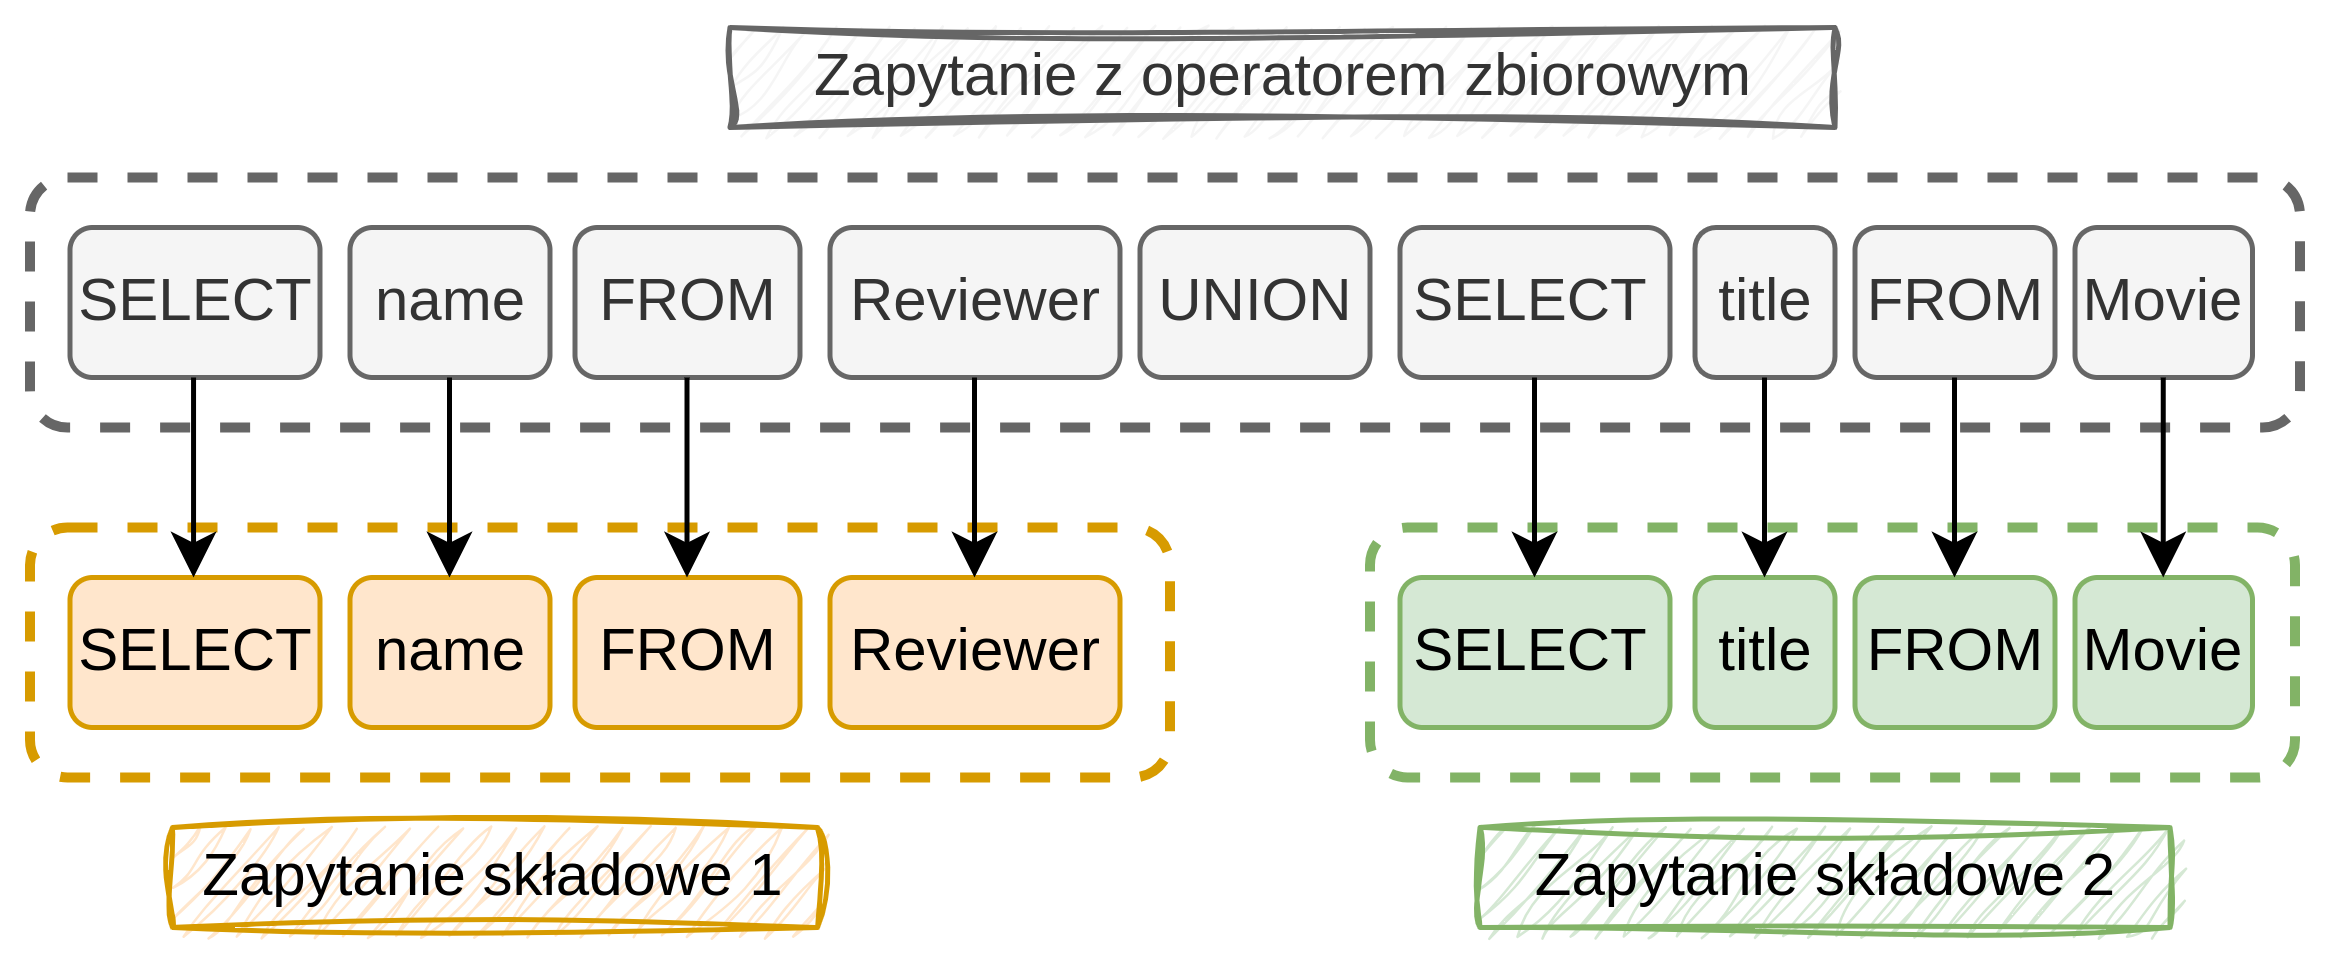
\includegraphics[width=1.0\linewidth]{images/query_decomposition_serial.png}
  \caption{Metoda dekomponowania zapytań z operatorami zbiorowymi}
  \label{fig:query-decomposition-serial}
\end{figure}

\begin{figure}[ht!]
  \centering
  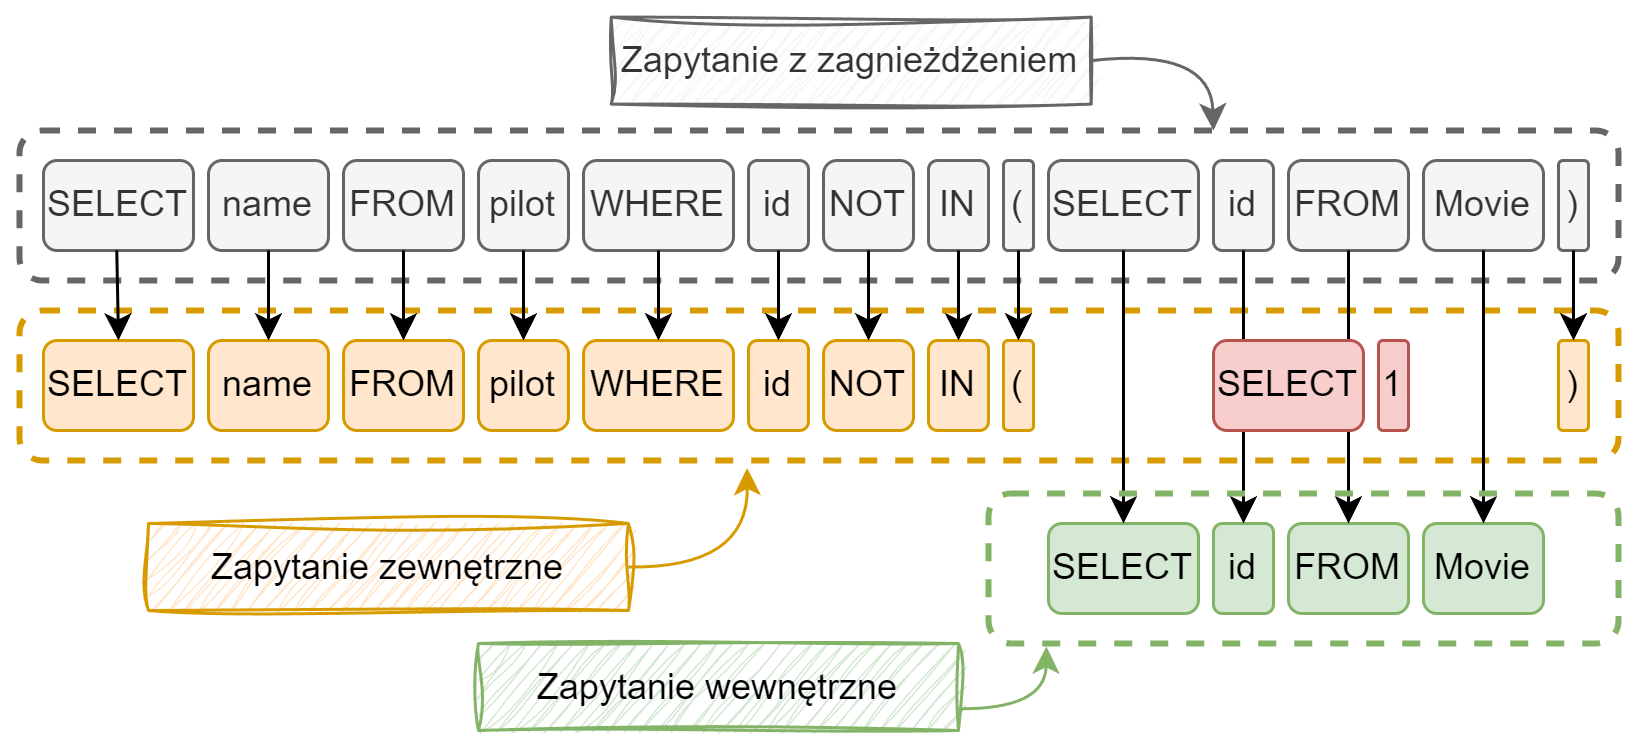
\includegraphics[width=1.0\linewidth]{images/query_decomposition_nested.png}
  \caption{Metoda dekomponowania zapytań z zagnieżdżeniem}
  \label{fig:query-decomposition-nested}
\end{figure}

\subsection{Rekonstrukcja informacji redundantnych}
Jak zostało wcześniej wskazane, dane źródłowe na których bazuje algorytm generacji zawierają jedynie informacje niezbędne. W finalnym zbiorze muszą zostać zawarte jednak dodatkowe informacje, które zostały uznane za redundantne, więc w danych źródłowych pominięte. Redundancja ta nie polega na dokładnych powtórzeniach, lecz na tym, że niektóre informacje stanowią pochodne innych, a skoro tak można je na tej podstawie zrekonstruować. Właśnie ten proces rekonstrukcji zostanie w tej części opisany.

Zdecydowaną część informacji do rekonstrukcji stanowią pytania oraz zapytania SQL podzielone na tokeny. Okazuję się, że duża część istniejących rozwiązań nie wykorzystuje tych informacji, ponieważ tokenizacji można dokonać na różne sposoby i wiele rozwiązań wykonuję ją samodzielnie, wybierając sposób dla siebie najkorzystniejszy. Nie mniej jednak pierwsze modele, jak i zapewne część nowszych, korzysta z dostarczonego w ramach zbioru sposobu tokenizacji, więc należy o ten aspekt zadbać.

\subsubsection{Tokenizacja pytań}
Pytania podzielone na tokeny występują w finalnych próbkach pod kluczem \code{question\_toks}. Tokenizacji postanowiono dokonać za pomocą dostarczonego w ramach biblioteki \code{spaCy} wielojęzycznego modelu. Wybrano akurat model wielojęzyczny, a nie polski, ponieważ dzięki temu skrypt nie będzie wprowadzał ograniczeń co do języka, a generowanie zbiorów z angielskimi pytaniami też się okazało w tej pracy przydatne. Porównano jednocześnie rezultaty tokenizacji polskich pytań za pomocą modelu wielojęzycznego oraz polskiego. Okazuję się, że wyniki różnią się jedynie w niewielkiej liczbie przypadków, co świadczy o tym, że model wielojęzyczny jest dość wysokiej jakości.

\subsubsection{Tokenizacja zapytań SQL}
Zapytania SQL podzielone na tokeny to kolejny element, który musi się znaleźć w finalnym zbiorze. Występuje on tam wewnątrz próbek pod postacią atrybutu \code{query\_toks}. Zaimplementowany sposób tokenizacji opiera się na początkowym znalezieniu w zapytaniu wszystkich wartości tekstowych. Wartości te są następnie tokenizowane za pomocą wspomnianego wcześniej wielojęzycznego modelu z biblioteki \code{spaCy}. Reszta zapytania jest natomiast rozbijana na elementy składowe z wykorzystaniem biblioteki \code{sqlparse}. Algorytm ten został zilustrowany na rysunku \ref{fig:query-tokenization}.

% TODO: Dodać coś o tym, że ten algorytm nie pokrywa się dokładnie ze zbiorem Spider

\begin{figure}[ht!]
  \centering
  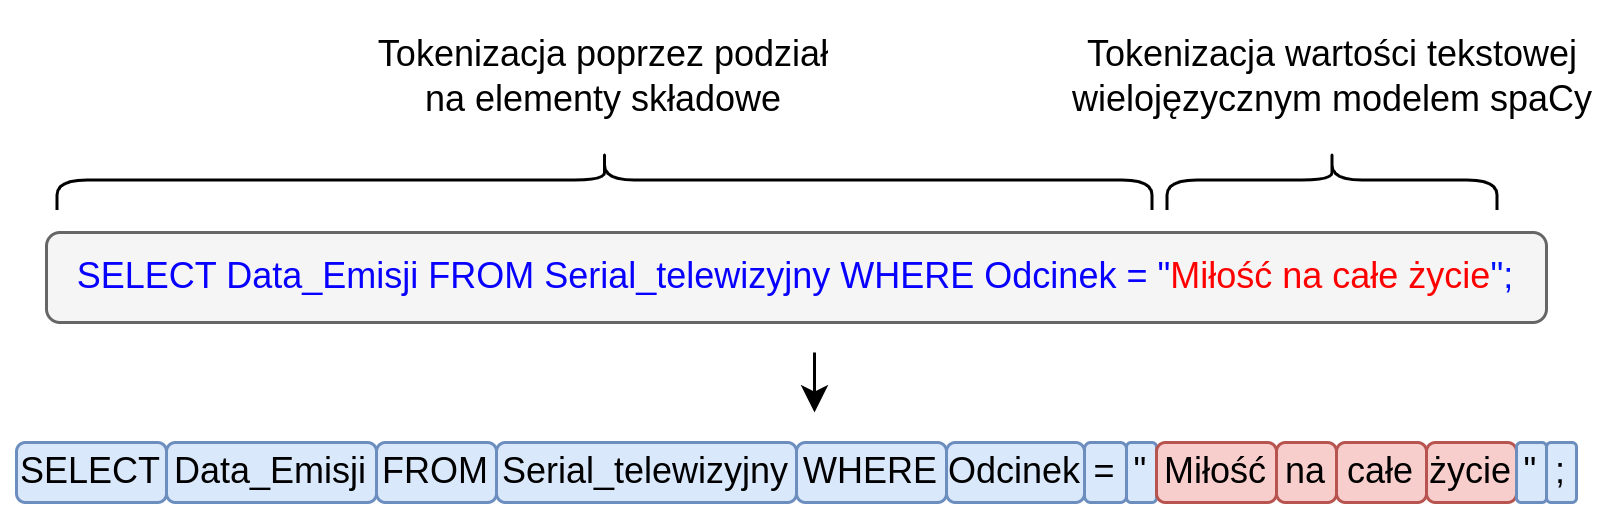
\includegraphics[width=1.0\linewidth]{images/query_tokenization.png}
  \caption{Schemat działania algorytmu tokenizacji zapytań SQL}
  \label{fig:query-tokenization}
\end{figure}

\subsubsection{Tokenizacja zapytań SQL bez wartości}
Próbki w zbiorze \code{Spider} posiadają atrybut o nazwie \code{query\_toks\_no\_value}, który powinien zawierać zapytanie SQL podzielone na tokeny, ale bez wartości, a dokładnie powinny one zostać zamaskowane za pomocą specjalnego tokena \code{value}. Została więc wykorzystana ta sama technika co do standardowej tokenizacji zapytań, lecz z tą różnicą, że znalezione w zapytaniu wartości zamiast podlegać rozbiciu na tokeny są po prostu zastępowane wspomnianym specjalnym tokenem. 

Opracowany algorytm jest niemal całkowicie zbieżny z wykorzystanym w oryginalnym zbiorze \code{Spider} sposobem tokenizacji. Aby to zweryfikować za jego pomocą dokonano podziału oryginalnych zapytań i sprawdzono, czy wyniki pokrywają się z oryginalnymi tokenami. Okazuję się, że różnice występują jedynie w 18 przypadkach spośród prawie dziesięciu tysięcy. Dokładniejsza analiza tych kilkunastu przykładów sugeruje, że zapytania SQL w nich zawarte zostały podzielone na tokeny w niekonsekwentny, odbiegające od reszty sposób, więc zbiór \code{Spider} nie jest do końca spójny. Brak spójności to jeden z problemów, którym rozwijana strategia generowania zbiorów ma przeciwdziałać i jak widać, problem ten jest rzeczywiście istotny.

\subsubsection{Parsowanie zapytań SQL}
Ważnym elementem, który musi się znaleźć w finalnym zbiorze, są odpowiednio sparsowane zapytania SQL. Występują one w próbkach pod kluczem \code{sql}. Tym razem istnieje publicznie dostępny skrypt, który dokonuje tego procesu. Zostały napotkane jednak pewne problemy wynikające z jego niedociągnięć. W jednym z pierwszych kroków dokonuje on bowiem wydobycia z zapytania aliasowania, czyli słownika mówiącego jakie występują w nim aliasy i na jakie tabele się mapują. Niestety dokonuje tego globalnie, a jak zostało przedyskutowane wcześniej, nie sprawdzi się to dla wszystkich zapytań, ponieważ występują w nich zakresy - w jednej części zapytania dany alias może mapować się na zupełnie inną tabelę niż w drugiej części. Podczas uruchamiana tego skrypt na zapytaniach ze zbioru \code{Spider} (co jest najczęstszym scenariuszem jego wykorzystania) nie zwraca on żadnych błędów. Przypuszcza się, że kłopotliwe zapytania zostały ręcznie poprawione, by stały się parsowalne. W przypadku jednak, gdy zapytania zostaną wcześniej poddane zmianie nazw tabel i kolumn, to problem ten wychodzi na wierzch i parsowanie kończy się najczęściej dla kilku zapytań niepowodzeniem. 

Nasuwające się rozwiązania powyższego problemu są dwa: można poprawić skrypt parsujący lub zmodyfikować plik mapowania nazw schematu tak, aby problem się nie ujawnił. Postanowiono wybrać drugą opcję, ponieważ nie wymaga ona wiele wysiłku w odróżnieniu od skomplikowanej naprawy skryptu. Przypuszcza się, że podobny był również sposób myślenia twórców zbioru \code{Spider} - zaimplementowali uproszczony skrypt parsujący, ponieważ koszt implementacji pełnego wariantu znacznie przewyższa koszt jednorazowego dostosowania kilkudziesięciu zapytań. Nie mniej jednak zauważone zachowanie zostało zgłoszone na platformie \code{GitHub} w odpowiednim repozytorium, by udokumentować i zwrócić uwagę na tą kwestię.

\section{Wykonywanie tłumaczenia}
W jednej z poprzednich części przedstawiony został w dogłębny sposób format danych źródłowych wykorzystywanych do generacji zbiorów. Zawiera on wiele fragmentów w których konieczne jest umieszczenie przetłumaczonego pytania, zapytania bądź nazwy. Kwestia tego w jaki sposób tłumaczenia te uzyskać została do tej pory w dużym stopniu przemilczana - zostanie to przedstawione w tej części.

\subsection{Wybór tłumacza}
Ważną do podjęcia decyzją jest wybór konkretnego narzędzie mającego być wykorzystanym do tłumaczenia maszynowego. Obecnie większość tego typu rozwiązań bazuje na uczeniu głębokim. Są one zazwyczaj zastrzeżone i dostęp do nich uzyskuje się za pomocą webowego API. Istnieją również narzędzia typu \code{open source}, które można uruchomić w całości na własnym urządzeniu. Pozwalają uniknąć naliczania kosztów i dają możliwość pewnej modyfikacji. Oferują za to mniejszą dokładność i dlatego postanowiono nie podążać tą drogą.

Podczas podejmowania ostatecznej decyzji wybór ograniczono do popularnych i renomowanych rozwiązań, takich jak \code{Google Cloud Translation API} \mycite{google-translation-api}, \code{Microsoft Azure AI Translator} \mycite{microsoft-translator}, \code{Amazon Translate API} \mycite{amazon-translator} oraz \code{DeepL} \mycite{deepl}. W szczególności to ostatnie wydaje się aktualnie wychodzić na prowadzenie pod względem jakości produkowanych tłumaczeń. Według informacji zawartych na swojej stronie \code{DeepL} generuje tłumaczenia ponad 3 razy dokładniejsze od rozwiązań konkurencji. Wysoką ich jakość potwierdzają również liczne artykuły naukowe \mycite{Yulianto2021}\mycite{Ternero2021}\mycite{Bahasa2023}, które powstały na fali zachwytu tym rozwiązaniem. Posiada on nawet dedykowaną bibliotekę do języka Python, ułatwiającą jego wykorzystanie. 

Jedynym aspektem, który może zniechęcać do wykorzystania \code{DeepL} są związane z tym koszty, nieco wyższe niż w przypadku konkurencyjnych rozwiązań. W czasie tworzenia niniejszej pracy podstawowy plan opierał się na bazowej opłacie w kwocie 20 złotych na miesiąc oraz dodatkowym obciążeniu wynoszącym prawie 90 złotych za każdy przetłumaczony milion znaków. Dostępny jest jednak również darmowy plan, pozwalający na przetłumaczenie pół miliona znaków każdego miesiąca za darmo.

\code{DeepL} został ostatecznie wybranym narzędziem, a głównym tego powodem jest niekwestionowana jakość produkowanych przez to narzędzie tłumaczeń. Oszacowano, że dostępne w ramach darmowego planu limity powinny pozwolić na zrealizowanie postawionych celów. Nie uda się to jednak w jeden miesiąc, a konieczne będzie rozłożenie tłumaczeń na dłuższy okres.

\subsection{Tłumaczenie nazw tabel i kolumn}
Okazuję się, że wysokiej jakości tłumaczenie nazw tabel i kolumn jest wyjątkowo trudnym zadaniem i z tego powodu zostało ono podzielone na dwa etapy. Pierwszy zakłada wykorzystanie tłumacza maszynowego, a drugi ręczne poprawienie tłumaczeń. To ostatnie nie polega jednak na przeglądaniu każdego przykładu jeden po drugim i szczegółowej walidacji, lecz na bardziej holistycznym i heurystycznym podejściu, które zostanie dokładnie opisane.

\subsubsection{Tłumaczenie maszynowe}
Jak zaznaczono wcześniej, w zbiorze \code{Spider} dla tabel i kolumn występują podwójne nazwy: oryginalnie występujące w bazie danych (\code{first\_name}) oraz w czytelnej, naturalnej postaci (\code{first name}). O ile przetłumaczenie tych ostatnich nie stanowi większego problemu, to nazwy oryginalne wymagają podjęcia dodatkowych akcji, ponieważ \code{DeepL} nie poradzi sobie z nimi w tej postaci - jako tłumaczenie zwróci te same nazwy, bez dokonywania żadnych zmian (\code{first\_name}), ponieważ potraktuje je jako nazwy własne, które nie podlegają tłumaczeniu. Zauważono, że \code{Google Cloud Translation} wykazuję pod tym kątem bardziej pożądane zachowanie, ale wciąż nie można na nim polegać. 

Aby poradzić sobie z zarysowanym problemem postanowiono przed tłumaczeniem dokonywać w nazwach podmiany znaków podkreślenia na spacje, by przekonwertować je do postaci naturalnej, a po tłumaczeniu spacje z powrotem zamieniać na znaki podkreślenia, co przedstawione zostało na rysunku \ref{fig:multi-word-translation}. Mechanizm ten nie sprawdził się dla wszystkich przypadków, ponieważ niektóre wielowyrazowe nazwy były zapisywane za pomocą innych konwencji niż oddzielanie słów znakiem podkreślenia. Były one jednak w mniejszości i tymi niedociągnięciami postanowiono się zająć na etapie ręcznych poprawek.

\begin{figure}[ht!]
  \centering
  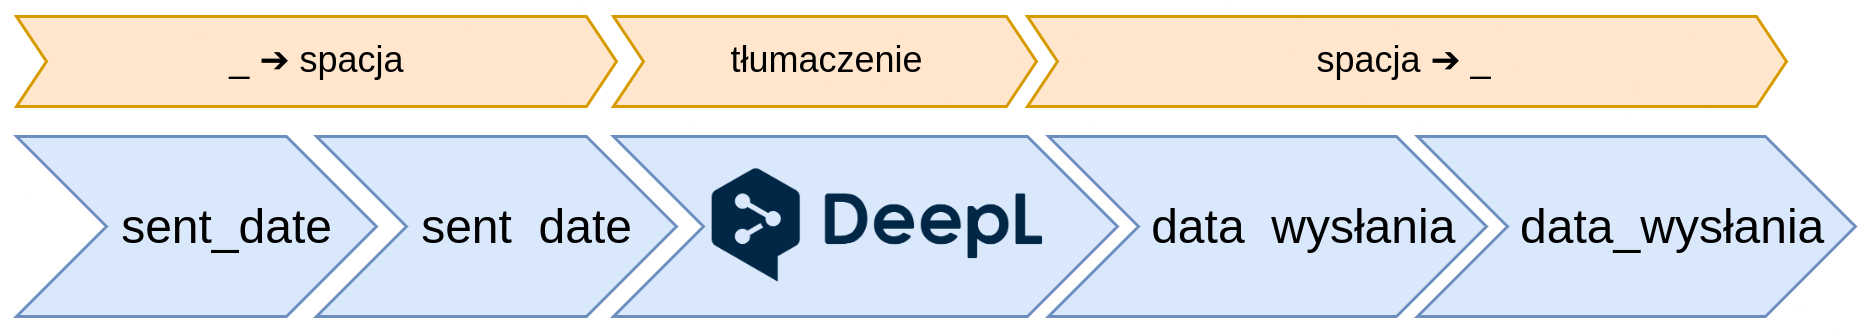
\includegraphics[width=1.0\linewidth]{images/multi_word_translation.png}
  \caption{Schemat algorytmu do tłumaczenia oryginalnych nazw tabel i kolumn}
  \label{fig:multi-word-translation}
\end{figure}

Podstawowa metoda tłumaczenia nazw to ich proste i intuicyjne przekazywanie do tłumacza. Jest to sposób, który został prawdopodobnie wykorzystany we wszystkich tłumaczeniach maszynowych zbioru \code{Spider}, ponieważ ich autorzy nie zwrócili szczególnej uwagi na tą kwestię. Podczas realizacji niniejszej pracy zauważono jednak, że wiele błędów w takich tłumaczeniach wynika z braku uwzględniania przez tłumacza kontekstu i opracowano metodę, która pozwala w dużej mierze obejść ten problem. Dla przykładu kolumna \code{home\_games} podstawową metodą jest tłumaczona jako \code{gry\_domowe}, natomiast ulepszona metoda kontekstowa weźmie pod uwagę, że kolumna ta znajduję się w tabeli \code{stadium} oraz bazie danych \code{game\_injury} i tym razem nazwa zostanie przetłumaczona poprawnie jako \code{mecze\_u\_siebie}.

Metoda kontekstowa polega na prostej obserwacji, że nowoczesne narzędzia bazujące na sieciach neuronowych, w szczególności \code{DeepL}, tłumaczą to samo słowo w różny sposób w zależności od kontekstu w jakim ono wystąpiło. Z tego powodu do tłumacza poza samymi nazwami tabel i kolumn postanowiono także podawać w roli kontekstu nazwy baz danych, a dla kolumn również nazwy tabeli. Zostały opracowane szablony, które służą do tworzenia skontekstualizowanych wyrażeń podawanych do tłumacza i wraz z przykładami użycia zostały przedstawione na rysunku \ref{fig:translation-in-context}. Dla porównania postanowiono dokonać tłumaczenia bezkontekstowego i okazało się, że wynikowe tłumaczenia nazw pomiędzy tymi metodami różnią się dla 21,41\% przypadków, co stanowi dużą różnicę.

\begin{figure}[ht!]
\centering
\begin{subfigure}{0.49\textwidth}
    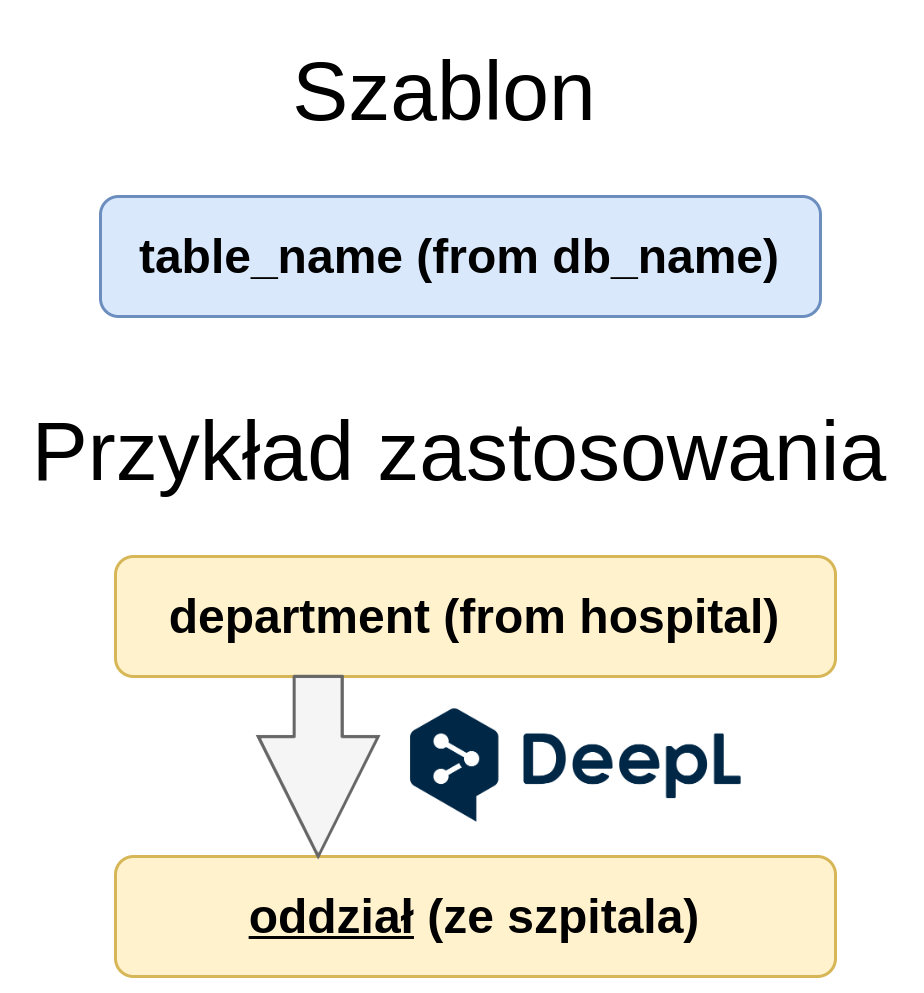
\includegraphics[width=\textwidth]{images/translation_in_context_table.png}
    \caption{Dla tabel}
    \label{fig:first}
\end{subfigure}
\hfill
\begin{subfigure}{0.49\textwidth}
    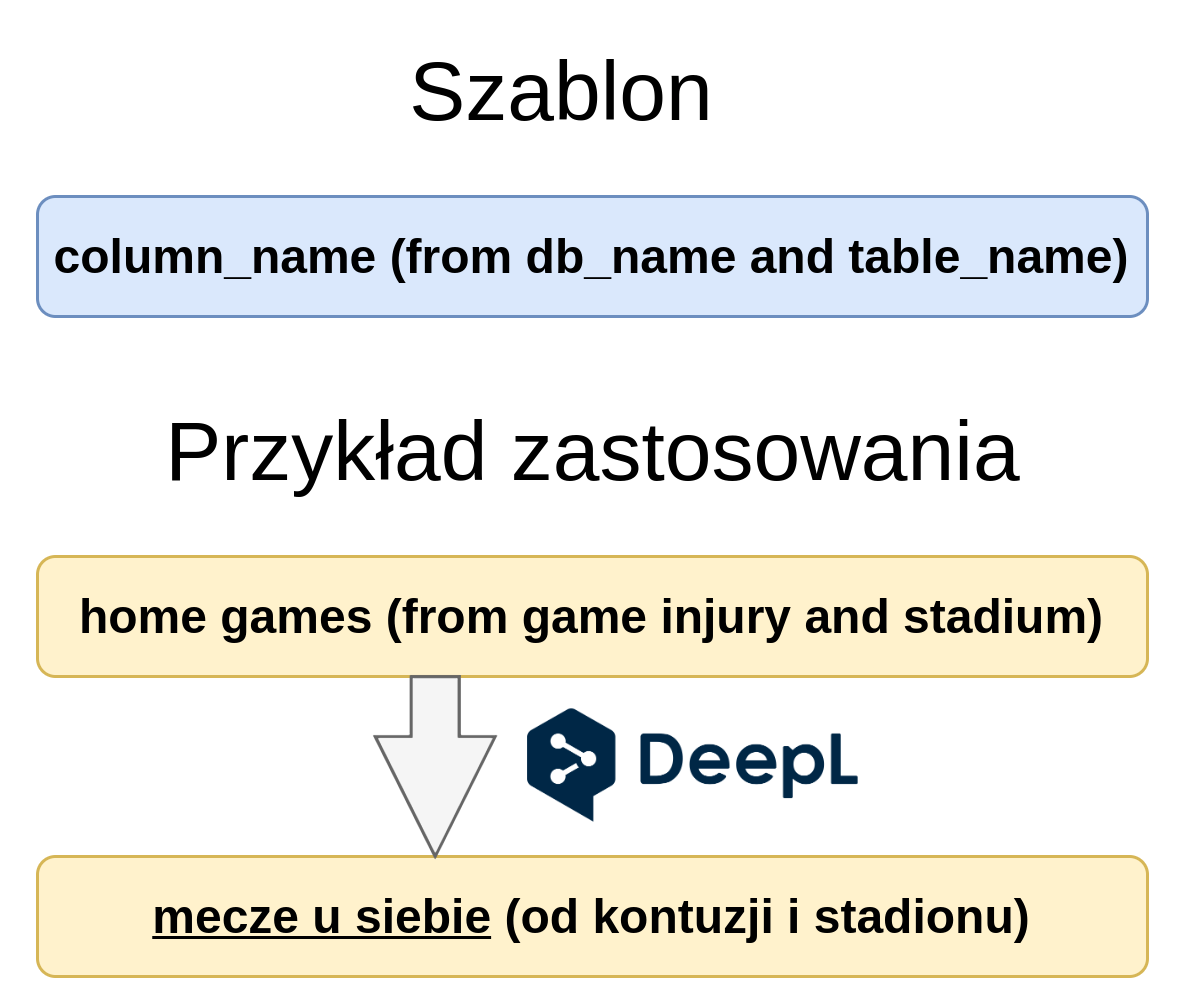
\includegraphics[width=\textwidth]{images/translation_in_context_column.png}
    \caption{Dla kolumn}
    \label{fig:second}
\end{subfigure}
\caption{Szablony do tłumaczenia kontekstowego}
\label{fig:translation-in-context}
\end{figure}

Przedstawiona strategia tłumaczenia kontekstowego jest zainspirowana metodą \code{SAVe}, opisaną w artykule dotyczącym wielojęzycznego zbioru \code{MultiSpider} \mycite{Dou2022}. Została tam wykorzystana jako metoda augmentacji w celu poprawienia osiąganych przez model wyników. Jest bardziej skomplikowana od przedstawionego powyżej wariantu, ponieważ zakłada wykorzystanie wielu szablonów oraz ma dodatkowy etap weryfikacji tłumaczeń, co jednak dla rozważanego problemu nie ma dobrego uzasadnienia.

Oczywistym minusem zaproponowanej metody jest istotne zwiększenie długości tekstów podawanych do tłumacza, co w przypadku \code{DeepL} wpływa na naliczenie wyższych kosztów, czy też szybsze wykorzystanie darmowych limitów - na co mimo wszystko się zdecydowano. Zaletą strategii kontekstowej jest poprawa tłumaczenia dla wielu nazw, jednak z pewnego punktu widzenia może ona także wpływać na obniżenie czytelności przetłumaczonego schematu. Zdarzają się bowiem przypadki, iż w obrębie jednej bazy danych pewna nazwa kolumny zostaje przetłumaczona na kilka różnych sposobów, chociaż nie powinna. Zmniejsza to spójność tak przetłumaczonego schematu, bo sugeruje, że przechowywane są w tych kolumnach dane o różnym znaczeniu, a w rzeczywistości jest inaczej. Nie jest więc banalnym oszacowanie wypadkowego wpływu zastosowania tej metody na jakość finalnego zbioru, uważa się jednak, że jest on pozytywny.

\subsubsection{Ręczne poprawki}
Po uzyskaniu tłumaczeń maszynowych nazw tabel i kolumn oraz ich wstępnej ocenie było oczywistym, że wciąż zawierają pewne błędy. Przejrzenie każdego z nich jedno po drugim wymagałoby znacznego nakładu czasu, więc postanowiono posłużyć się metodami heurystycznymi, by zlokalizować tylko te najbardziej podejrzane. 

Zauważono, że dla błędnych tłumaczeń bardzo często nazwa przetłumaczona jest identyczna z angielską, więc korzystając z tego faktu, prostych skryptów oraz możliwości edytora \code{Visual Studio Code} dokonano znalezienia właśnie takich przypadków, a następnie je poprawiono. Były to w dużej mierze nazwy składające się z kilku wyrazów połączonych ze sobą za pomocą innej konwencji niż znaki podkreślenia, bo tylko ten najpopularniejszy wariant był obsługiwany w fazie maszynowej. Dość częste były również kilkuliterowe skróty jak \code{mid} (movie id), czy \code{aid} (author id), z którymi - co nie dziwi - \code{DeepL} sobie nie poradził. Poza tym dokonano poprawy kilkunastu wyrażeń w przypadku których zaobserwowano częste pomyłki, jak tłumaczenie \code{name} na \code{imię i nazwisko}, chociaż powinno zostać przetłumaczone jako \code{nazwa}, czy \code{id}, które niepotrzebnie zostało przetłumaczone na rozwlekłą nazwę \code{identyfikator}.

Na cały etap ręcznych poprawek zostało poświęcone kilka godzin i w jego wyniku zmodyfikowano 10,54\% tłumaczeń maszynowych. Wydaje się to dużą częścią, lecz większość z tych modyfikacji dokonano w szybki, półautomatyczny sposób.


\subsection{Tłumaczenie pytań}
Tłumaczenie pytań sprowadza się do uzupełnienia w przedstawionym wcześniej formacie danych źródłowych wartości \code{question.pl} na podstawie atrybutu \code{question.en}. W tym przypadku pytania zostały bezpośrednio przekazane do tłumacza, bez stosowania żadnych dodatkowych sztuczek. Uznano, że stosowanie tłumaczenia kontekstowego, które oznaczałoby rozszerzenie przekazywanych do tłumacza tekstów o nazwę bazy danych z której pochodzą, nie ma sensu. Wiązałoby się to z tłumaczeniem większej liczby znaków na podstawie których \code{DeepL} obciąża swoich użytkowników, a uzyskana poprawa prawdopodobnie nie byłaby znacząca. Pytania są bowiem zwykle na tyle długie, że pozwalają tłumaczowi na wywnioskowanie domeny której dotyczą, więc wybranie odpowiednich tłumaczeń dla problematycznych słów nie stanowi już tak dużego problemu.

Etap manualnych poprawek nie został w tym przypadku wykorzystany, gdyż pytania zawierają dużą ilość tekstu i ciężko jest dostrzec w nich ewentualne błędy. Nie znaleziono również żadnych sposobów na znalezienie podejrzanych tłumaczeń, czy dokonanie półautomatycznych poprawek, tak jak to miało miejsce dla tłumaczenia nazw tabel i kolumn. Ostatecznie maszynowe tłumaczenia pytań wydawały się na tyle wysokiej jakości, że postanowiono przejść do kolejnych etapów.

\subsection{Tłumaczenie wartości w zapytaniach SQL}
Tłumaczenie wartości w zapytaniach SQL odbywa się poprzez uzupełnienie atrybutów \code{query.pl} na podstawie \code{query.en} w pliku danych źródłowych o przedstawionym wcześniej formacie. Ten ostatni atrybut zawiera oryginalne zapytania SQL, natomiast pierwszy zapytania z wszelkimi anglojęzycznymi łańcuchami znaków przetłumaczonymi na język polski.

W celu znalezienia w danym zapytaniu wartości tekstowych dokonywano jego przetwarzania z wykorzystaniem biblioteki \code{sqlparse}. Pozwalała ona podzielić zapytanie na poszczególne tokeny i wybrać te, które posiadają typ \code{Token.Literal.String}, czyli właśnie wartości tekstowe. Są to wyrażenia zamknięte w pojedynczych lub podwójnych cudzysłowach, które przekazywano do \code{DeepL} w celu uzyskania tłumaczeń, a następnie zastępowano nimi oryginalne teksty. Wyjątek stanowią jedynie wartości występujące w roli szablonów po słowie kluczowym \code{LIKE}, takie jak \code{'\%Hey\%'}, \code{'\%East\%'}, \code{'S\%'}. Nie są one zapisane w języku naturalnym, ponieważ zawierają specjalne znaki, stanowiące problem dla tłumacza maszynowego. Z tego względu, a także biorąc pod uwagę rzadkość takich przypadków, postanowiono przetłumaczyć je manualnie. Wizualizacja tego etapu została przedstawiona na rysunku \ref{fig:value-translation}.

\begin{figure}[ht!]
  \centering
  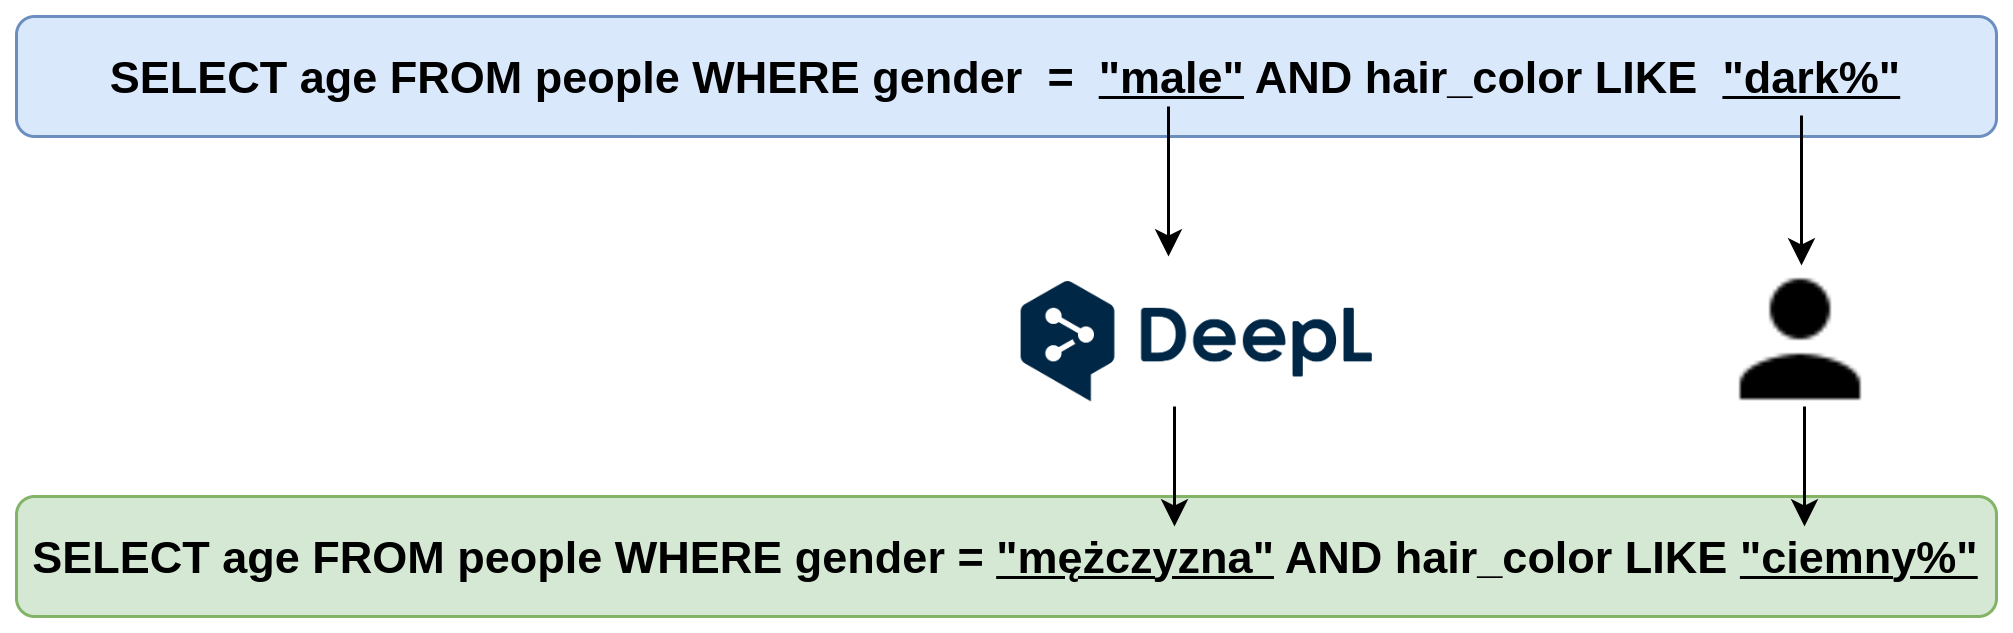
\includegraphics[width=1.0\linewidth]{images/value_translation.png}
  \caption{Wizualizacja etapu tłumaczenia wartości w zapytaniach SQL}
  \label{fig:value-translation}
\end{figure}

\section{Stworzone zbiory}
Niniejszy podrozdział stanowi ukoronowanie pracy nad polskimi zbiorami danych, ponieważ zawiera ich ostateczne przedstawienie wraz 
z analizą. Zgodnie z obraną strategią kompletne zbiory stanowią połączenie jednego z bazowych zbiorów oraz jednego z mapowań nazw tabel i kolumn, dlatego komponenty te zostaną opisane osobno. Na koniec kilka ich połączeń zostanie nazwanych w celu ułatwienia dalszych rozważań.

% Niniejszy podrozdział stanowi ukoronowanie pracy nad polskimi zbiorami danych, ponieważ zawiera on przedstawienie i analizę przygotowanych zbiorów przykładów, tłumaczeń schematów oraz ostatecznie zbiorów, które poprzez ich kombinację można wygenerować.

\subsection{Zbiory bazowe}
Przygotowanych zostało pięć bazowych zbiorów z których zdecydowanie najistotniejszym ze względu na swoją renomę oraz powszechne wykorzystanie jest \code{Spider}. W celu weryfikacji i porównywania trenowanych modeli przetłumaczone zostały także zbiory \code{Spider-DK} oraz \code{Spider-Syn}. \code{CoSQL} oraz \code{SParC} to natomiast znacznie różniące się od swoich oryginałów zbiory, które przygotowano i przetłumaczono głównie w celu uzyskania dodatkowych danych treningowych.

\begin{table}[ht]
    \centering
    \begin{tabular}{|l|R{0.15\textwidth}|R{0.15\textwidth}|R{0.15\textwidth}|}
        \hline
        \thead{Zbiór} & \thead{Część\\treningowa} & \thead{Część\\walidacyjna} & \thead{Razem} \\
        \hline
        Spider & 8659 & 1034 & 9693 \\
        \hline
        Spider-DK & 0 & 535 & 535 \\
        \hline
        Spider-Syn & 3556 & 773 & 4329 \\
        \hline
        CoSQL & 1562 & 230 & 1792 \\
        \hline
        SParC & 2651 & 366 & 3017 \\
        \hhline{|=|=|=|=|} 
        Razem & 16428 & 2938 & 19366 \\
        \hline
    \end{tabular}
    \caption{Zestawienie liczby próbek w poszczególnych zbiorach}
    \label{tab:samples-count}
\end{table}

W tabeli \ref{tab:samples-count} przedstawione zostały liczności próbek we wszystkich stworzonych zbiorach bazowych z uwzględnieniem podziału na części treningowe oraz walidacyjne. \code{Spider} to zbiór najliczniejszy z którego żadne próbki nie były usuwane i dokładnie odpowiadają oryginalnym. Drugim największym jest \code{Spider-Syn}, który zawiera przykłady ze \code{Spider} z niewielkimi modyfikacjami, lecz w wyniku usuwania duplikatów skurczył się o ponad połowę. Zbiory \code{SParC} oraz \code{CoSQL} są następne w kolejności i one również w czasie deduplikacji zostały uszczuplone. Najmniejszym zbiorem, posiadającym jedynie część walidacyjną, jest \code{Spider-DK}, chociaż z niego żadne próbki usuwane nie były.

\begin{table}[ht]
    \centering
    \begin{tabular}{|l|R{0.15\textwidth}|R{0.15\textwidth}|R{0.15\textwidth}|R{0.15\textwidth}|R{0.15\textwidth}|}
        \hline
        \thead{Zbiór} & \thead{Easy} & \thead{Medium} & \thead{Hard} & \thead{Extra} \\
        \hline
        Spider & 2231 (23\%) & 3445 (36\%) & 2095 (22\%) & 1922 (20\%) \\
        Spider-DK & 110 (21\%) & 246 (46\%) & 74 (14\%) & 105 (20\%) \\
        Spider-Syn & 952 (22\%) & 1825 (42\%) & 884 (20\%) & 668 (15\%) \\
        CoSQL & 949 (53\%) & 488 (27\%) & 222 (12\%) & 133 (\s7\%) \\
        SParC & 2131 (71\%) & 706 (23\%) & 138 (\s5\%) & 42 (\s1\%) \\
        \hline
        Wszystkie & 6373 (33\%) & 6710 (35\%) & 3413 (18\%) & 2870 (15\%) \\
        \hline
    \end{tabular}
    \caption{Zestawienia liczby próbek o poszczególnych poziomach trudności}
    \label{tab:difficulty}
\end{table}

Repozytorium zbioru \code{Spider} dostarcza algorytm pozwalający przypisać do każdego zapytania SQL jeden z następujących czterech poziomów trudności: \code{Easy}, \code{Medium}, \code{Hard} oraz \code{Extra hard}. Postanowiono to wykorzystać w celu analizy rozłożenia zapytań o poszczególnych poziomach trudności we wszystkich stworzonych zbiorach. Wyniki tej analizy umieszczono w tabeli \ref{tab:difficulty}. Można je podsumować twierdzeniem, że najbardziej skomplikowane zapytania występują w zbiorze \code{Spider}, co niewątpliwie jest istotnym powodem jego popularności. Niemal równie trudne zapytania posiada zbiór \code{Spider-DK}, lecz jest on wielokrotnie mniejszy. Z drugiej strony wyjątkowo proste okazały się zapytania znajdujące się w oryginalnie kontekstowych zbiorach \code{CoSQL} oraz \code{SParC}.

\begin{table}[ht]
    \centering
    \begin{tabular}{|l|P{0.20\textwidth}|P{0.20\textwidth}|}
        \hline
        \thead{Zbiór} & \thead{Pytania (en/pl)} & \thead{Wartości (en/pl)} \\
        \hline
        Spider & 66,74 / 66,44 & 10,66 / 11,28 \\
        Spider-DK & 66,01 / 65,93 & \s8,47 / \s8,59 \\
        Spider-Syn & 74,03 / 74,14 & 9,65 / 10,28 \\
        CoSQL & 53,05 / 52,66 & 10,11 / 10,72 \\
        SParC & 44,94 / 45,52 & 10,24 / 10,84 \\
        \hline
        Wszystkie & 63,69 / 63,61 & 10,32 / 10,94 \\
        \hline
    \end{tabular}
    \caption[Zestawienie liczby znaków w pytaniach i wartościach]{Zestawienie liczby znaków w pytaniach i wartościach dla języka angielskiego i polskiego}
    \label{tab:questions-lengths}
\end{table}

Interesującą analizą, której postanowiono dokonać, jest zestawienie długości tekstów angielskich oraz przetłumaczonych na język polski. Zgodnie z danymi ukazanymi w tabeli \ref{tab:questions-lengths} średnie długości wszystkich pytań liczone w znakach różnią się zaledwie o 0,08. W przypadku długości wartości tekstowych różnica ta jest nieco większa i wynosi 0,61. Wzrost może być spowodowany faktem, że występują one jedynie w niektórych próbkach i ze statystycznego punktu widzenia miara ta jest mniej pewna. Mimo wszystko różnice okazały się zdecydowanie mniejsze od spodziewanych, co pokazuję, że język polskim nie różni się znacznie od angielskiego pod kątem zwięzłości.

\subsection{Mapowania nazw}
Zgodnie z przedstawionymi do tej pory treściami opracowane zostały dwie główne drogi dokonywania tłumaczeń nazw tabel i kolumn: metoda bezkontekstowa oraz uważana za lepszą metoda kontekstowa. Mapowania uzyskane z wykorzystaniem tych strategii nazwano odpowiednio \code{pl\_nocontext} oraz \code{pl\_context}. W tłumaczeniach maszynowych uzyskanych metoda kontekstową dokonano następnie dużej liczby półautomatycznych poprawek i uzyskane w ten sposób mapowanie nazwano \code{pl\_context\_curated}. Istnieje oczywiście także mapowanie, które zachowuje angielskie nazwy, które określono jako \code{en\_original}.

Wymienione mapowania zawierają polskie znaki, które jednak rzadko są spotykane w praktyce, więc opracowano skrypt, który dokonuje ich zastąpienia występującymi w kodowaniu \code{ASCII} odpowiednikami, jak \code{wysokość -> wysokosc}. W ten sposób powstały odpowiadające trzem wcześniej wspomnianym mapowania z sufiksem \code{\_sanitized}. Schemat przedstawiający naszkicowane zależności został przedstawiony na rysunku \ref{fig:mappings}.

\begin{figure}[ht!]
  \centering
  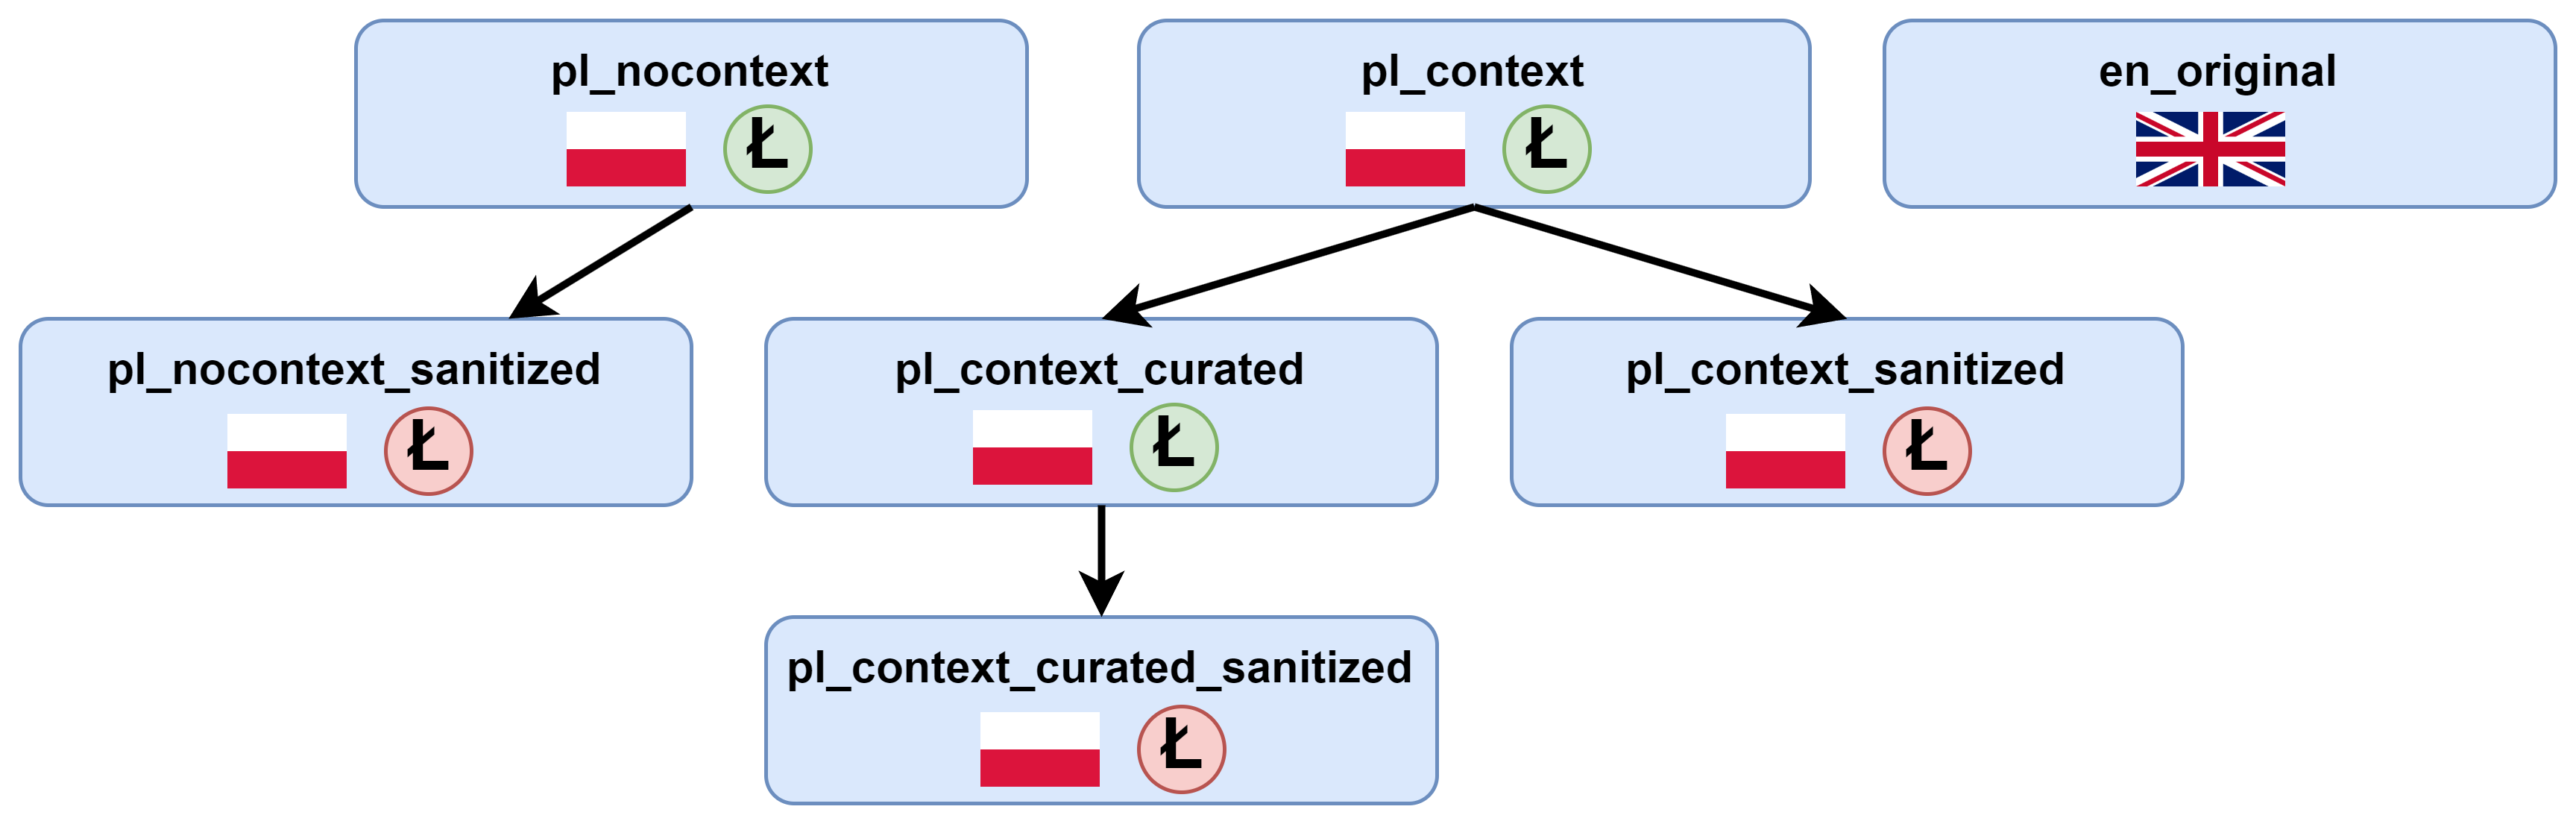
\includegraphics[width=1.0\linewidth]{images/mappings.png}
  \caption{Schemat zależności pomiędzy stworzonymi mapowaniami nazw}
  \label{fig:mappings}
\end{figure}

Podobnie jak to było w przypadku pytań, tutaj również postanowiono zbadać w jaki sposób zastosowanie poszczególnych mapowań wpływa na długość finalnych nazw tabel i kolumn. Wyniki tej analizy przedstawiono w tabeli \ref{tab:names-lengths}. Można zauważyć, że tłumaczenie na język polski zwiększa długości o około jeden znak, co stanowi prawie 10\%. Jest to znaczny wzrost, biorąc pod uwagę, że w przypadku tłumaczenia pytań był on marginalny. Wyjaśniać może to obserwacja, że angielskie nazwy tabel i kolumn często bywają zapisywane skrótowo, ponieważ pomijane są choćby przyimki, a tłumaczenia produkowane przez \code{DeepL} są bardziej opisowe i takie elementy już zawierają.

\begin{table}[ht]
    \centering
    \begin{tabular}{|l|c|c|c|c|}
        \hline
        \multirow{2}{*}[-6pt]{\thead{Mapowanie}} &
        \multicolumn{2}{c|}{\thead{Tabele}} &
        \multicolumn{2}{c|}{\thead{Kolumny}} \\
        \cline{2-5}
        \multirow{2}{*}{} &
        \thead{name} &
        \thead{name\_original} &
        \thead{name} &
        \thead{name\_original} \\
        \hline
        \code{en\_original} & 10,48 & 10,28 & 10,26 & \s9,87 \\
        \code{pl\_nocontext} & 11,37 & 11,17 & 11,24 & 10,83 \\
        \code{pl\_context } & 11,46 & 11,23 & 11,38 & 11,11 \\
        \code{pl\_context\_curated} & 11,55 & 11,29 & 11,36 & 11,07 \\
        \hline
    \end{tabular}
    \caption{Zestawienie średniej liczby znaków w mapowaniach nazw}
    \label{tab:names-lengths}
\end{table}

\subsection{Nazwane warianty}

W celu ułatwienia dalszej pracy poprzez możliwość odwoływania się do konkretnych zbiorów kilka ich konfiguracji zostało nazwanych. Ponadto zdefiniowane zostały pewne połączenia tych zbiorów, ponieważ występują do nich częste odwołania.

\begin{figure}[ht!]
  \centering
  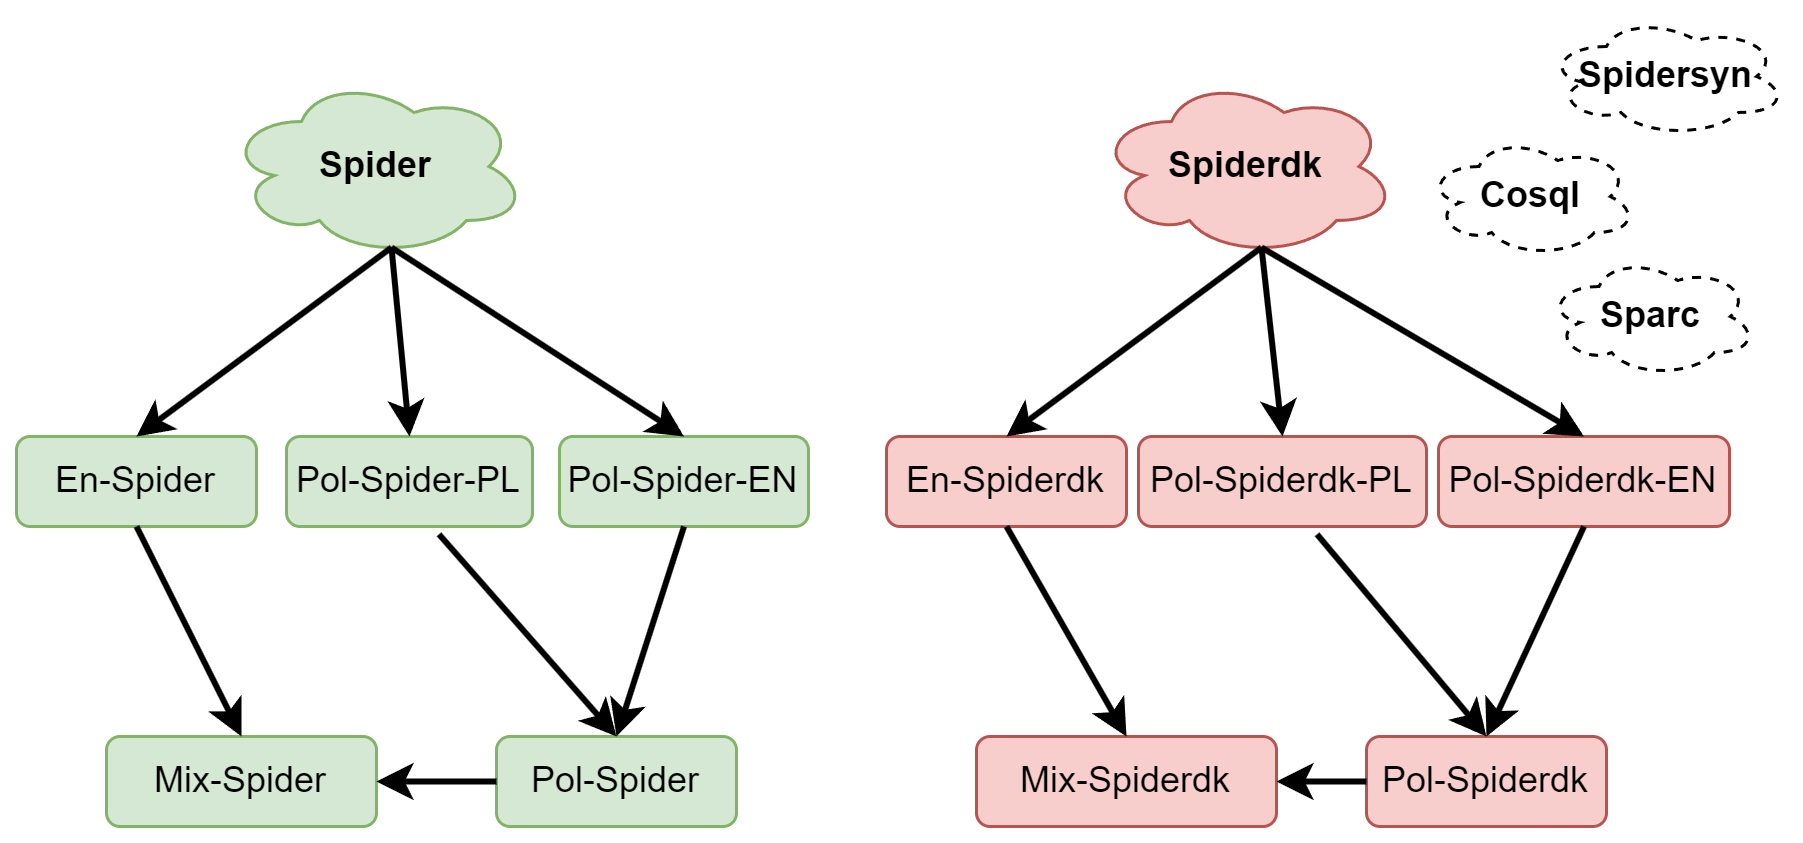
\includegraphics[width=1.0\linewidth]{images/datasets.png}
  \caption{Schemat zależności pomiędzy zbudowanymi zbiorami danych}
  \label{fig:datasets}
\end{figure}

Schemat zdefiniowanych zbiorów został przedstawiony na rysunku \ref{fig:datasets}. Można z niego odczytać, że na bazie zbioru \code{Spider} wygenerowane zostały trzy zbiory pochodne. \code{En-Spider} to wariant całkowicie angielski, bardzo podobny do oryginalnego \code{Spider}, ale z minimalnymi różnicami, jak sposób tokenizacji. Wykorzystuje angielskie pytania i wartości oraz mapowanie \code{en\_original}. Kolejny to \code{Pol-Spider-PL}, czyli wariant polski z polskim schematem baz danych, uzyskanym za pomocą mapowania \code{pl\_context\_curated\_sanitized}. Trzecim jest natomiast \code{Pol-Spider-EN}, czyli również zbiór polski, ale z angielskim schematem baz danych, stworzonym za pomocą mapowania \code{en\_original}.

Opracowany został dodatkowo skrypt, który pozwala na łatwe łączenie zbiorów. Za jego pomocą dokonano połączenia dwóch wspomnianych polskich wariantów w zbiór, który nazwano \code{Pol-Spider}. Ma on podwójny rozmiar i obejmuje dwojaki sposób nazewnictwa kolumn i tabel. Jest istotny z praktycznego punktu widzenia, ponieważ nie ogranicza się tylko do pierwszego, czy drugiego przypadku, lecz obejmuje obie powszechnie spotykane konwencje. Po rozszerzeniu tego już rozbudowanego polskiego zbioru o angielski \code{En-Spider} powstaje natomiast \code{Mix-Spider}, czyli dość nietypowy zbiór zawierający próbki w obu językach.

Podobny schemat nazewnictwa do przedstawionego powyżej został zastosowany do reszty zbiorów bazowych, czyli \code{Spider-DK}, \code{Spider-Syn}, \code{CoSQL} oraz \code{SParC}. Wykorzystano wymowne i schematyczne nazwy, aby ułatwić ich zapamiętanie. Możliwych do wygenerowania konfiguracji zbiorów jest znacznie więcej, lecz do tych przedstawionych będą występowały częstsze odwołania.
